\documentclass[a4paper]{article}
\usepackage{student}
\usepackage{graphicx}
\usepackage{caption}
\usepackage[version=4]{mhchem}
\usepackage{tikz}
\usetikzlibrary{shapes.geometric, arrows.meta, positioning, decorations.pathreplacing}
\usepackage{enumitem}
\usepackage{tikz-3dplot}
\usepackage{multicol}
\usepackage{longtable}
\usepackage{amsmath}
\usepackage{booktabs}

\tikzstyle{arrow} = [thick,->,>=stealth]

% Definindo o estilo de destaque com linhas pontilhadas
\tikzstyle{highlight} = [draw, dashed, thick, rectangle, rounded corners, inner sep=0.2cm, orange]


\tikzstyle{startstop} = [
rectangle, rounded corners, minimum width=0.5cm,
text centered, draw=black, fill=blue!10, font=\small
]
\tikzstyle{startstop_S} = [
rectangle, rounded corners, minimum width=0.5cm, minimum height=0.8cm,
text centered, draw=black, fill=green!30, font=\small
]
\tikzstyle{decision} = [
diamond, aspect=2, draw=black, fill=orange!15, align=center,
text centered, inner sep=0pt, font=\small
]
\tikzstyle{decision_S} = [
diamond, aspect=2, draw=black, fill=orange!30, align=center,
text centered, inner sep=0pt, font=\small
]
\tikzstyle{arrow} = [thick,->,>=stealth]



% Metadata
\date{\today}
\setmodule{PGF5261/IFUSP: Teoria de Grupos Aplicada a Sólidos e Moléculas. Prof.: Lucy Assali} 
\setterm{1o. semestre, 2025}

%-------------------------------%
% Other details
% TODO: Fill these
%-------------------------------%
\title{Exercício 04 - 17/06}
\setmembername{Nara Avila Moraes}  % Fill group member names
\setmemberuid{5716734}  % Fill group member uids (same order)

%-------------------------------%
% Add / Delete commands and packages
% TODO: Add / Delete here as you need
%-------------------------------%
\usepackage{amsmath,amssymb,bm}

\newcommand{\KL}{\mathrm{KL}}
\newcommand{\R}{\mathbb{R}}
\newcommand{\E}{\mathbb{E}}
\newcommand{\T}{\top}

\newcommand{\expdist}[2]{%
\normalfont{\textsc{Exp}}(#1, #2)%
}
\newcommand{\expparam}{\bm \lambda}
\newcommand{\Expparam}{\bm \Lambda}
\newcommand{\natparam}{\bm \eta}
\newcommand{\Natparam}{\bm H}
\newcommand{\sufstat}{\bm u}

% Main document
\begin{document}
% Add header
\header{}

\textbf{Questão 1.}
Considere as simetrias do íon Carbonato \ce{CO3^{2-}} e responda os seguintes ítems:

\begin{center}
	\begin{minipage}{1\textwidth}
		\centering
		\includegraphics[width=1\textwidth]{figuras/ion_carbonato.png} 
		\captionof{figure}{Íon Carbonato}
	\end{minipage}
	\hfill
	\begin{minipage}{1\textwidth}
		\begin{itemize}
			\item[(1.1)] Identifique o \textbf{grupo de simetria} do Íon.
			\item[(1.2)] Encontre as \textbf{representações irredutíveis} associadas às \textbf{translações}, \textbf{rotações} e às \textbf{vibrações da molécula}.
			\item[(1.3)] Tente associar as representações irredutíveis vibracionais com os \textbf{modos de vibração}: stretching modes e bending modes;
			\item[(1.4)] encontrar os \textbf{modos ativos no infravermelho} considerando que a absorção ocorre a partir do estado vibracional fundamental que pertence à representação irredutível totalmente simétrica;
			\item[(1.5)] encontrar os \textbf{modos ativos no Raman} considerando que a transição entre estados vibracionais ocorra a partir do estado vibracional fundamental (pertencente à RI totalmente simétrica).
		\end{itemize}
	\end{minipage}
\end{center}

\begin{answer}[Ítem 1.1 - Grupo de Simetria da Molécula]
\vspace{1em}

%%%%%%%%%%%%%%%%%%%%%%%%%%%%%%%%%%%%%%%%%%%%%%%%%%%%%%%%%%%%%%%%
%                              E
%%%%%%%%%%%%%%%%%%%%%%%%%%%%%%%%%%%%%%%%%%%%%%%%%%%%%%%%%%%%%%%%
\begin{itemize}[noitemsep, topsep=0pt, label=--]
        \begin{minipage}[t]{0.48\textwidth}
			      \centering
			      \includegraphics[width=5cm, height=5cm, keepaspectratio,clip]{figuras/E.png}
			      \captionof{figure}{Simetria \(E\)}
		      \end{minipage}
		      \hfill
		      \begin{minipage}[t]{0.48\textwidth}
			      \centering
			      \includegraphics[width=5cm, height=5cm, keepaspectratio,clip]{figuras/E.png}
			      \captionof{figure}{Operação \( E \) aplicada}
		      \end{minipage}
        \begin{align*}
        \textbf{:} \quad 
                E(1,2,3,4)                 & = (1,2,3,4) \\
        \end{align*}

%%%%%%%%%%%%%%%%%%%%%%%%%%%%%%%%%%%%%%%%%%%%%%%%%%%%%%%%%%%%%%%%
%                              C3
%%%%%%%%%%%%%%%%%%%%%%%%%%%%%%%%%%%%%%%%%%%%%%%%%%%%%%%%%%%%%%%%

        \begin{minipage}[t]{0.48\textwidth}
        \vspace{0.4em}
			      \centering
			      \includegraphics[width=5cm, height=5cm, keepaspectratio,clip]{figuras/C3.png}
			      \captionof{figure}{Eixo de rotação \(C_3\)}
		      \end{minipage}
		      \hfill
		      \begin{minipage}[t]{0.48\textwidth}
                      \vspace{0.4em}
			      \centering
			      \includegraphics[width=5cm, height=5cm, keepaspectratio,clip]{figuras/C3_1.png}
			      \captionof{figure}{Operação \( C_3 \) aplicada}
		      \end{minipage}
        \begin{align*}\textbf{:} \quad 
                C_3(1,2,3,4)               & = (1,4,2,3) \\
                C_3^2(1,2,3,4)             & = (1,3,4,2)  \\
        \end{align*}

%%%%%%%%%%%%%%%%%%%%%%%%%%%%%%%%%%%%%%%%%%%%%%%%%%%%%%%%%%%%%%%%
%                              C2
%%%%%%%%%%%%%%%%%%%%%%%%%%%%%%%%%%%%%%%%%%%%%%%%%%%%%%%%%%%%%%%%
        \begin{minipage}[t]{0.48\textwidth}
			      \centering
			      \includegraphics[width=5cm, height=5cm, keepaspectratio,clip]{figuras/C2.png}
			      \captionof{figure}{Eixo de rotação \(C_2^{(a)}\)}
		      \end{minipage}
		      \hfill
		      \begin{minipage}[t]{0.48\textwidth}
			      \centering
			      \includegraphics[width=5cm, height=5cm, keepaspectratio,clip]{figuras/C2_1.png}
			      \captionof{figure}{Operação \( C_2^{(a)} \) aplicada}
		      \end{minipage}
              
        \begin{align*}\textbf{:} \quad 
            C_2^{(a)}(1,2,3,4)         & = (1,2,4,3) \\
            C_2^{(b)}(1,2,3,4)         & = (1,4,3,2)  \\
            C_2^{(c)}(1,2,3,4)         & = (1,3,2,4) \\
        \end{align*}
        
%%%%%%%%%%%%%%%%%%%%%%%%%%%%%%%%%%%%%%%%%%%%%%%%%%%%%%%%%%%%%%%%
%                              sigma v
%%%%%%%%%%%%%%%%%%%%%%%%%%%%%%%%%%%%%%%%%%%%%%%%%%%%%%%%%%%%%%%%
        \begin{minipage}[t]{0.48\textwidth}
			      \centering
			      \includegraphics[width=5cm, height=5cm, keepaspectratio,clip]{figuras/sigma_v.png}
			      \captionof{figure}{Plano de reflexão \(\sigma_{v1}\)}
		      \end{minipage}
		      \hfill
		      \begin{minipage}[t]{0.48\textwidth}
			      \centering
			      \includegraphics[width=5cm, height=5cm, keepaspectratio,clip]{figuras/sigma_v_1.png}
			      \captionof{figure}{Operação \(\sigma_{v1} \) aplicada}
		      \end{minipage}
        \begin{align*}\textbf{:} \quad 
            \sigma_{v1}(1,2,3,4)       & = (1,2,4,3) \\
            \sigma_{v2}(1,2,3,4)       & = (1,4,3,2) \\
            \sigma_{v3}(1,2,3,4)       & =  (1,3,2,4) \\
        \end{align*}

%%%%%%%%%%%%%%%%%%%%%%%%%%%%%%%%%%%%%%%%%%%%%%%%%%%%%%%%%%%%%%%%
%                              sigma h
%%%%%%%%%%%%%%%%%%%%%%%%%%%%%%%%%%%%%%%%%%%%%%%%%%%%%%%%%%%%%%%%
        \begin{minipage}[t]{0.48\textwidth}
			      \centering
			      \includegraphics[width=5cm, height=5cm, keepaspectratio,clip]{figuras/sigma_h.png}
			      \captionof{figure}{Plano de reflexão \(\sigma_{h}\)}
		      \end{minipage}
		      \hfill
		      \begin{minipage}[t]{0.48\textwidth}
			      \centering
			      \includegraphics[width=5cm, height=5cm, keepaspectratio,clip]{figuras/sigma_h_1.png}
			      \captionof{figure}{Operação \(\sigma_{h} \) aplicada}
		      \end{minipage}
              
        \begin{align*}\textbf{:} \quad 
                \sigma_h(1,2,3,4)          & = (1,2,3,4) \\
        \end{align*}

%%%%%%%%%%%%%%%%%%%%%%%%%%%%%%%%%%%%%%%%%%%%%%%%%%%%%%%%%%%%%%%%
%                              S_3
%%%%%%%%%%%%%%%%%%%%%%%%%%%%%%%%%%%%%%%%%%%%%%%%%%%%%%%%%%%%%%%%
        \begin{minipage}[t]{0.31\textwidth}
			      \centering
			      \includegraphics[width=5cm, height=5cm, keepaspectratio,clip]{figuras/C3.png}
			      \captionof{figure}{Eixo de rotação \(C_{3}\)}
		      \end{minipage}
		      \hfill
		      \begin{minipage}[t]{0.31\textwidth}
			      \centering
			      \includegraphics[width=5cm, height=5cm, keepaspectratio,clip]{figuras/C3_sigmah.png}
			      \captionof{figure}{Plano de reflexão \(\sigma_h \) }
		      \end{minipage}
              \begin{minipage}[t]{0.31\textwidth}
			      \centering
			      \includegraphics[width=5cm, height=5cm, keepaspectratio,clip]{figuras/S3_1.png}
			      \captionof{figure}{Operação \(S_{3} \) aplicada}
		      \end{minipage}
        \begin{align*}\textbf{:} \quad 
            S_3(1,2,3,4)               & = (1,4,2,3)\\
            S_3^5(1,2,3,4)             & = (1,3,4,2)
        \end{align*}
	\end{itemize}

Conforme ilustrado nas figuras, o íon carbonato apresenta as seguintes simetrias:

\begin{itemize}
    \item \textbf{Um eixo de rotação $C_{3}$}, passando pelo centro do carbono, perpendicular ao plano que contém os oxigênios. Com rotações de $120^\circ$ e $240^\circ$.

    \item \textbf{Três eixos de rotação $C_{2}$}, todos perpendiculares ao eixo $C_{3}$, passando por cada par de O-C. Estes eixos estão espaçados de $120^\circ$ entre si ao redor do eixo principal. Com rotacões de $180^\circ$ cada.

    \item \textbf{Três planos de reflexão verticais $\sigma_{v}$}, cada um contendo o eixo $C_{3}$ e passando por um oxigênio e entre os dois oxigênios opostos.

    \item \textbf{Um plano de reflexão horizontal $\sigma_{v}$} passando por todas os átomos do íon.

    \item \textbf{Duas rotações impróprias $S_{3}$}, correspondentes à combinação de uma reflexão por um plano $\sigma_{h}$ perpendicular ao eixo da rotação seguida de rotação $C_{3}$. Rotações impróprias de $120^\circ$ e $240^\circ$.

\end{itemize}


Portanto, conforme demonstrado no fluxograma de classificação, o grupo de simetria do íon carbonato é o \textbf{$D_{3h}$}.

	\begin{center}
		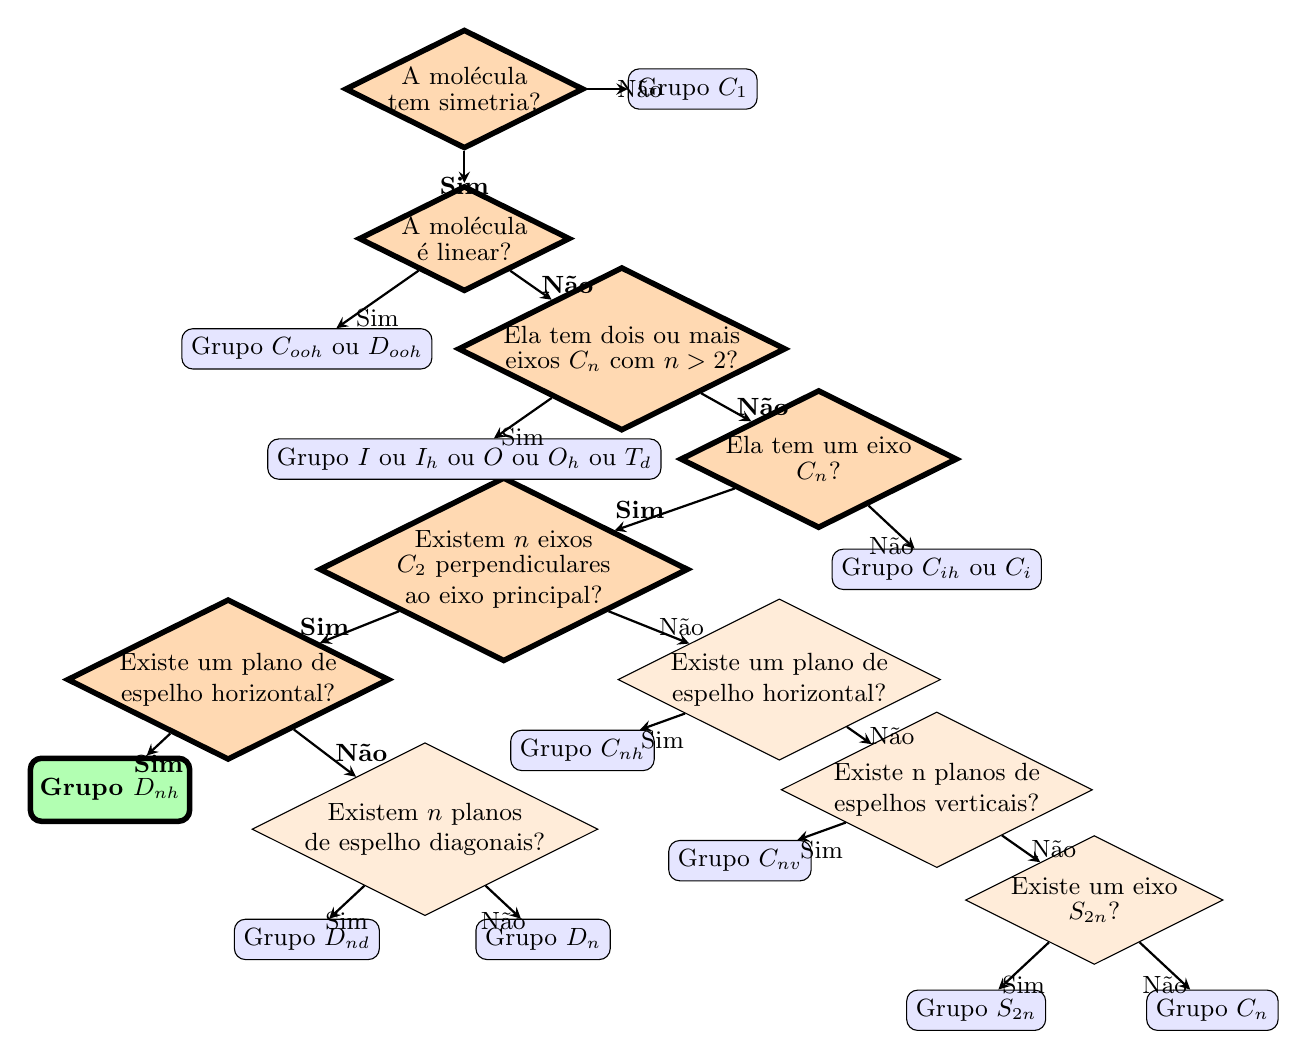
\begin{tikzpicture}[node distance=1.4cm]
			% Nodes de decisao
			\node (Q_1) [decision_S, xshift=-7cm, line width=0.7mm] {\shortstack{A molécula\\tem simetria?}};
			\node (Q_2) [decision_S, below of=Q_1, yshift=-0.5cm, line width=0.7mm] {\shortstack{A molécula\\é linear?}};
			\node (Q_4) [decision_S, below of=Q_2, xshift=2cm, line width=0.7mm] {\shortstack{Ela tem dois ou mais\\eixos \( C_n \) com \( n>2 \)?}};
			\node (Q_6) [decision_S, below of=Q_4, xshift=2.5cm, line width=0.7mm] {\shortstack{Ela tem um eixo\\\( C_n \)?}};
			\node (Q_9) [decision_S, below of=Q_6, xshift=-4cm, line width=0.7mm] {\shortstack{Existem \( n \) eixos\\\( C_2 \) perpendiculares\\ao eixo principal?}};
			\node (Q_10) [decision_S, below of=Q_9, xshift=-3.5cm, line width=0.7mm] {\shortstack{Existe um plano de\\espelho horizontal?}};
			\node (Q_11) [decision, below of=Q_10, xshift=2.5cm, yshift=-0.5cm] {\shortstack{Existem \( n \) planos\\de espelho diagonais?}};
			\node (Q_12) [decision, below of=Q_9, xshift=3.5cm] {\shortstack{Existe um plano de\\espelho horizontal?}};
			\node (Q_13) [decision, below of=Q_12, xshift=2cm] {\shortstack{Existe n planos de\\espelhos verticais?}};
			\node (Q_14) [decision, below of=Q_13, xshift=2cm] {\shortstack{Existe um eixo\\\( S_{2n} \)?}};

			% Nodes finais
			\node (CooDoo) [startstop, below of=Q_2, xshift=-2cm] {Grupo $C_{ooh}$ ou $D_{ooh}$};
			\node (G_alta_simetria) [startstop, below of=Q_4, xshift=-2cm] {Grupo $I$ ou $I_h$ ou $O$ ou $O_h$ ou $T_d$};
			\node (G_baixa_simetria) [startstop, below of=Q_6, xshift=1.5cm] {Grupo $C_{ih}$ ou $C_i$};
			\node (Dnh) [startstop_S, below of=Q_10, xshift=-1.5cm, line width=0.7mm] {\textbf{Grupo $D_{nh}$}};
			\node (Dnd) [startstop, below of=Q_11, xshift=-1.5cm] {Grupo $D_{nd}$};
			\node (Dn) [startstop, below of=Q_11, xshift=1.5cm] {Grupo $D_n$};
			\node (Cnv) [startstop, below of=Q_13, xshift=-2.5cm, yshift=0.5cm] {Grupo $C_{nv}$};
			\node (Cnh) [startstop, below of=Q_12, xshift=-2.5cm, yshift=0.5cm] {Grupo $C_{nh}$};
			\node (S2n) [startstop, below of=Q_14, xshift=-1.5cm] {Grupo $S_{2n}$};
			\node (Cn) [startstop, below of=Q_14, xshift=1.5cm] {Grupo $C_n$};
			\node (C1) [startstop, right of=Q_1, xshift=1.5cm] {Grupo $C_1$};

			% Connections
			\draw [arrow] (Q_1) -- node[anchor=north, font=\small] {\textbf{Sim}} (Q_2);
			\draw [arrow] (Q_2) -- node[anchor=west, font=\small] {\textbf{Não}} (Q_4);
			\draw [arrow] (Q_4) -- node[anchor=west, font=\small] {\textbf{Não}} (Q_6);
			\draw [arrow] (Q_6) -- node[anchor=east, font=\small] {\textbf{Sim}} (Q_9);
			\draw [arrow] (Q_9) -- node[anchor=east, font=\small] {\textbf{Sim}} (Q_10);
			\draw [arrow] (Q_10) -- node[anchor=west, font=\small] {\textbf{Não}} (Q_11);
			\draw [arrow] (Q_9) -- node[anchor=west, font=\small] {Não} (Q_12);
			\draw [arrow] (Q_12) -- node[anchor=west, font=\small] {Não} (Q_13);
			\draw [arrow] (Q_13) -- node[anchor=west, font=\small] {Não} (Q_14);

			% Final Connections
			\draw [arrow] (Q_2) -- node[anchor=north, font=\small] {Sim} (CooDoo);
			\draw [arrow] (Q_4) -- node[anchor=north, font=\small] {Sim} (G_alta_simetria);
			\draw [arrow] (Q_6) -- node[anchor=north, font=\small] {Não} (G_baixa_simetria);
			\draw [arrow] (Q_10) -- node[anchor=north, font=\small] {\textbf{Sim}} (Dnh);
			\draw [arrow] (Q_11) -- node[anchor=north, font=\small] {Sim} (Dnd);
			\draw [arrow] (Q_11) -- node[anchor=north, font=\small] {Não} (Dn);
			\draw [arrow] (Q_12) -- node[anchor=north, font=\small] {Sim} (Cnh);
			\draw [arrow] (Q_13) -- node[anchor=north, font=\small] {Sim} (Cnv);
			\draw [arrow] (Q_14) -- node[anchor=north, font=\small] {Sim} (S2n);
			\draw [arrow] (Q_14) -- node[anchor=north, font=\small] {Não} (Cn);
			\draw [arrow] (Q_1) -- node[anchor=west, font=\small] {Não} (C1);

		\end{tikzpicture}
	\end{center}
\end{answer}

\begin{answer}[Ítem 1.2 - Representações irredutíveis associadas às translações, rotações e vibrações]
Para encontrar as representações irredutíveis associadas às translações, rotações e vibrações do íon carbonato \ce{{CO}3^{2-}}, precisamos calcular a representação \(\Gamma_{mov}\) da molécula considerando todos os graus de liberdade em que esse movimento reside. A movimentação de cada átomo contribui com 3 graus de liberdade (x, y, z), sendo a representação da movimentação do íon tem no total dimensão:
\[
dim(\Gamma_{mov})= 3 + 3 + 3 + 3 = 12
\]
Para calcular a representação dos movimentos da molécula, precisamos avaliar como cada operação de simetria do grupo \( D_{3h} \) age sobre os vetores \( x, y, z \) de cada átomo, adotando a origem de cada sistema cartesiano localizada em cada um dos átomos de carbono em sua posição de equilíbrio. O objetivo é obter os caracteres \( \chi(R) \) da representação \( \Gamma_{\text{mov}} \), que corresponde ao traço da matriz de representação associada à operação \( R \).

O caractere \( \chi(R) \) de uma operação \( R \) é igual ao número de coordenadas \( x, y, z \) que permanecem invariantes ou inversas (com sinal negativo), ou o valor de suas projeções nos seus eixos originais sob essa operação.

\vspace{1em}
\textbf{Operação \( E \)}

Todas as coordenadas de todos os átomos se mantém invariantes e portanto o \( \chi(E) \) é igual a 12.

\vspace{1em}
\textbf{Operação \( C_{3} \)}

Aplicando a operação \( C_3 \), todos os átomos de oxigênio mudam de sítio, o que quer dizer que não contribuem para o traço da matriz da operação. Analisando o átomo de carbono, sob operação \( C_3 \) os eixos x e y são rotacionados em          \(120^{\circ}\) cada e o eixo z se mantém inalterado.

\[
R_{xy}(120^\circ) =
\begin{bmatrix}
\cos(120^\circ) & -\sin(120^\circ) \\
\sin(120^\circ) & \cos(120^\circ)
\end{bmatrix}
=
\begin{bmatrix}
-1/2 & -\sqrt{3}/2 \\
\sqrt{3}/2 & -1/2
\end{bmatrix}
\]

\[
\text{Tr}(R_{xy}) = \cos(120^\circ) + \cos(120^\circ) = -\frac{1}{2} - \frac{1}{2} = -1
\]

O traço da operação \( C_3 \) para este íon é então a soma dos traços não nulos que resulta em -1 + 1 = 0.

\vspace{1em}
\textbf{Operação \( C_{2} \)}

Nesta operação se escolhemos o eixo de rotação em x de um dos oxigênios e do carbono, a rotação fará com que os dois outros oxigênios restantes mudem de sítio o que faz com que não haja contribuição deles para o traço da operação. 

Analisando o oxigênio e o carbono que passam pelo eixo de rotação, em ambos, o eixo x se mantém inalterado, contribuindo com +2 para o traço, enquanto em ambos o eixo z e y invertem de sinal, contribuindo com -4. 

Portanto o traço da operação \( C_{2} \) para este íon é +2 - 4 = -2.

\vspace{1em}
\textbf{Operação \( \sigma_{h} \)}

Nesta operação nenhum átomo muda de sítio, e portanto todos contribuem de forma não nula para o traço. Em cada átomo o eixo z inverte de posição, contribuindo com -4, e o eixo x e y em cada átomo continuam invariantes, contribuindo com +8. 

Portanto o traço da operação \( \sigma_{h} \) para este íon é - 4 + 8 = 4.

\vspace{1em}
\textbf{Operação \( S_{3} \)}

Nesta operação todos os oxigênios mudam de sítio e portanto não contribuem com o traço. Analisando o carbono central, os eixos x e y sofrem rotação de \(120^\circ\) e o eixo z sofre uma inversão.

O traço resultante da rotação já foi demonstrado ter o valor de -1, e a inversão do eixo z contribui com -1, resultando em -2.

\vspace{1em}
\textbf{Operação \( \sigma_{v} \)}

Nesta operação, dois oxigênios mudam de sítio e não contribuem para o traço. Analisando o oxigênio e o carbono pertencentes ao plano de reflexão, temos que os eixos do plano não se alteram, contribuindo com +4, enquanto o eixo perpendicular ao plano é invertido, contribuindo com -2. 

Portanto o traço da operação \( \sigma_{h} \) para este íon é + 4 - 2 = 2.

\vspace{2em}
Obtivemos então os seguintes caracteres para \( \Gamma_{\text{mov}} \):

\[
\Gamma_{\text{mov}} = 
\begin{array}{c|cccccc}
\text{Classe} & E & 2C_3 & 3C_2' & \sigma_h & 2S_3 & 3\sigma_v \\
\hline
\chi          & 12 & 0 & -2 & 4 & -2 & 2 \\
\end{array}
\]

Os 3N graus de liberdade podem ser decompostos da seguinte forma:

\[
\Gamma^{(3N)} = \Gamma_{\text{trans}}^{(3)} \oplus \Gamma_{\text{rot}}^{(3)} \oplus \Gamma_{\text{vib}}^{(3N-6)}
\]

Para identificar qual a representação irredutível dos modos são de \textbf{translação}, \textbf{rotação} ou \textbf{vibração}, vamos primeiro identificar a representação de \(\Gamma_{(mov)}\) em termo das representações irredutíveis do grupo \(D_{3h}\) de acordo com a tabela de caracteres do grupo:

\[
\begin{array}{c|cccccc|c|c}
D_{3h} & E & 2C_3 & 3C_2' & \sigma_h & 2S_3 & 3\sigma_v & \text{Linear/Angular} & \text{Quadrático} \\
\hline
A_1'  & 1 & 1 & 1 & 1 & 1 & 1 &  & x^2 + y^2,\ z^2 \\
A_2'  & 1 & 1 & -1 & 1 & 1 & -1 & R_z &  \\
E'    & 2 & -1 & 0 & 2 & -1 & 0 & (x,\ y) & x^2 - y^2,\ xy \\
A_1'' & 1 & 1 & 1 & -1 & -1 & -1 &  &  \\
A_2'' & 1 & 1 & -1 & -1 & -1 & 1 & z &  \\
E''   & 2 & -1 & 0 & -2 & 1 & 0 & (R_x,\ R_y) & xz,\ yz \\
\hline
\Gamma_{\text{mov}} & 12 & 0 & -2 & 4 & -2 & 2 & & \\
\end{array}
\]

\subsection*{Decomposição da Representação \( \Gamma_{\text{mov}} \)}

A decomposição em representações irredutíveis é feita usando a fórmula:

\[
a_\alpha = \frac{1}{h} \sum_{g} \chi^{(\Gamma)}(g) \cdot \chi^{(\alpha)}(g)^* \cdot n_g
\]

Com \( h = 12 \), obtemos:

\begin{align*}
a_{A_1'} &= \frac{1}{12} (1 \cdot 12 + 1 \cdot 0 + 1 \cdot 0 + 1 \cdot 0 + 1 \cdot 0 + 1 \cdot 2) = 1 \\
a_{A_2'} &= \frac{1}{12} (1 \cdot 12 + 1 \cdot 0 + (-1) \cdot 0 + 1 \cdot 0 + 1 \cdot 0 + (-1) \cdot 2) = 1 \\
a_{A_2''} &= \frac{1}{12} (1 \cdot 12 + 1 \cdot 0 + (-1) \cdot 0 + (-1) \cdot 0 + (-1) \cdot 0 + 1 \cdot 2) = 2 \\
a_{E'} &= \frac{1}{12} (2 \cdot 12 + (-1) \cdot 0 + 0 \cdot 0 + 2 \cdot 0 + (-1) \cdot 0 + 0 \cdot 2) = 3 \\
a_{E''} &= \frac{1}{12} (2 \cdot 12 + (-1) \cdot 0 + 0 \cdot 0 + (-2) \cdot 0 + 1 \cdot 0 + 0 \cdot 2) = 1
\end{align*}

\subsection*{Resultando}

\[
\Gamma_{\text{mov}} = A_1' \oplus A_2' \oplus 2A_2'' \oplus 3E' \oplus E''
\]

As translações são movimentos lineares de x, y, e z, enquanto as rotações são movimentos em torno de \(R_x\), \(R_y\) e \(R_z\). Separando esses modos pela tabela de caracteres, econtramos que:


\[
\Gamma_{\text{trans}}^{(3)} =  A_2'' \oplus E'
\]

e 

\[
\Gamma_{\text{rot}}^{(3)} =  A_2' \oplus E''
\]

E portanto os modos de vibração são os modos restantes:

\[
\Gamma_{\text{vib}}^{(4)} = A_1' \oplus A_2'' \oplus 2E'
\]

\end{answer}

\begin{answer}[Ítem 1.3 - Modos de vibração]

Os modos stretching estão associados a mudanças de comprimentos das ligações, enquanto os modos bending estão associados a mudanças nos ângulos entre as ligações.


A decomposição da representação de movimento forneceu os seguintes modos vibracionais:

\[
\Gamma_{\text{vib}} = A_2' \oplus A_2'' \oplus 2E'
\]

Com base na tabela de caracteres do grupo $D_{3h}$, é possível identificar os comportamentos físicos associados a cada representação irredutível:

\begin{itemize}
  \item \textbf{$A_2'$}: Esta representação não transforma como nenhum vetor cartesiano direto ($x$, $y$, $z$), mas aparece frequentemente associada a \textbf{flexões angulares simétricas no plano} ($xy$). Portanto, associamos este modo a um \textbf{bending simétrico no plano}, em que os ângulos entre as ligações C–O variam de forma simétrica.
  
  \item \textbf{$A_2''$}: Representa transformação segundo o eixo $z$, mas não está associada a translação ou rotação (já removidas). Em moléculas planas como o íon carbonato, este modo está relacionado a \textbf{distorções fora do plano}, onde os oxigênios oscilam para cima e para baixo em relação ao plano molecular. Logo, este é um \textbf{modo de bending fora do plano}.

  \item \textbf{$2E'$}: Representações duplas como $E'$ correspondem a modos degenerados bidimensionais. Neste caso, temos dois modos:
    \begin{itemize}
      \item Um dos modos $E'$ está associado a \textbf{stretching assimétrico} das ligações C–O, onde dois comprimentos aumentam e um diminui, ou vice-versa, mantendo o centro de massa fixo.
      \item O outro modo $E'$ representa \textbf{bending degenerado no plano}, ou seja, variações dos ângulos O–C–O de forma assimétrica.
    \end{itemize}
\end{itemize}
\end{answer}

\begin{answer}[Ítem 1.4 - Modos ativos no Infravermelho]



Os modos vibracionais ativos no infravermelho são aqueles cuja representação irredutível está associada às transformações dos vetores cartesianas $x$, $y$, $z$, ou seja, $E'$ e $A_2''$. Como a decomposição vibracional do íon carbonato é:
\[
\Gamma_{\text{vib}} = A_2' \oplus A_2'' \oplus 2E'
\]
os modos ativos no IV são:
\[
\boxed{A_2'' \quad \text{e} \quad 2E'}
\]





\end{answer}

\begin{answer}[Ítem 1.5 - Modos ativos no Raman]

Os modos ativos no \textbf{Raman} são aqueles cujas representações estão associadas aos termos quadráticos da polarizabilidade ($x^2 + y^2$, $xy$, $z^2$, etc), ou seja, $A_1'$, $E'$, e $E''$. Dentre os modos vibracionais presentes, apenas $E'$ aparece na lista de modos Raman-ativos. Assim, os modos ativos no Raman são:
\[
\boxed{2E'}
\]

\end{answer}

\end{document}